\documentclass{beamer}

\usepackage{xcolor}
\usepackage[latin1]{inputenc}
\usepackage{pgfplots}
\usepackage{tikz}
\usetikzlibrary{shapes,arrows,calc,positioning,shadows,fillbetween}

%%%<
\usepackage{verbatim}
\usepackage[active,tightpage]{preview}


\PreviewEnvironment{tikzpicture}
\setlength\PreviewBorder{5pt}%
%%%>

\usepackage[outline]{contour}
\contourlength{0pt}

\begin{document}
\pagestyle{empty}

\pgfdeclarelayer{background layer}
\pgfsetlayers{background layer,main}

\definecolor{bl}{rgb}{0, 0.4470, 0.7410}
\definecolor{ye}{rgb}{    0.9290    0.6940    0.1250}


\pgfdeclarelayer{background layer}
\pgfsetlayers{background layer,main}

  \pgfplotsset{
    every mark/.append style={solid}
  }

% Define block styles
\tikzstyle{water} = [rectangle, draw, fill=bl!60,minimum height=2em, inner sep = 0]
\tikzstyle{solvent} = [rectangle, draw, fill=ye!60, minimum height=2em, inner sep = 0]
\tikzstyle{line} = [draw, -latex', line width = 2pt]
% \tikzstyle{cloud} = [draw, ellipse,fill=re!20, node distance=3cm,
% minimum height=2em]
% \tikzstyle{primitive} = [draw, isosceles triangle, line width = 1pt,rotate = 20]
% \tikzstyle{fragment} = [circle, draw, minimum size = 15pt, inner sep = 0pt]

\begin{tikzpicture}
  \node[anchor=south west,inner sep=0] (krG) at (-5,-5) {
    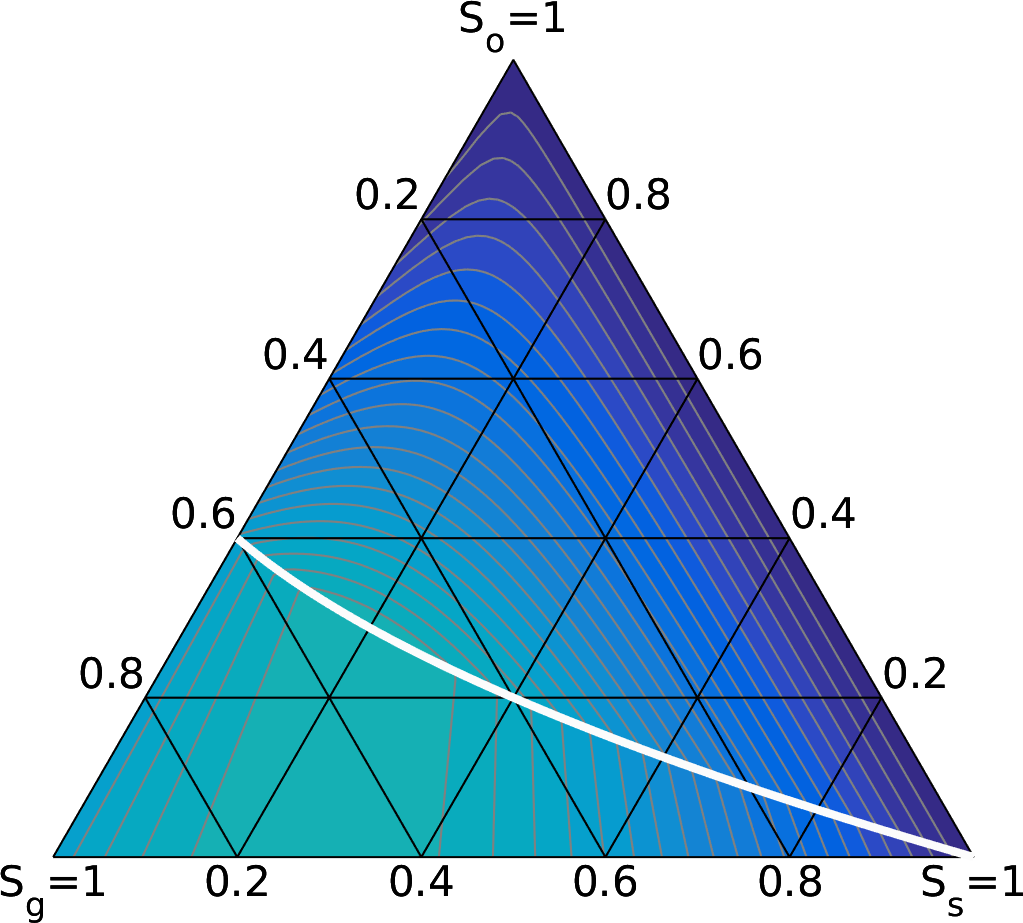
\includegraphics[width = 0.6\textwidth]{krG.png}};
  \node at (-1.8,-5.5) {Gas relperm};
  \node[anchor=south west,inner sep=0] (krS) at (5,-5) {
    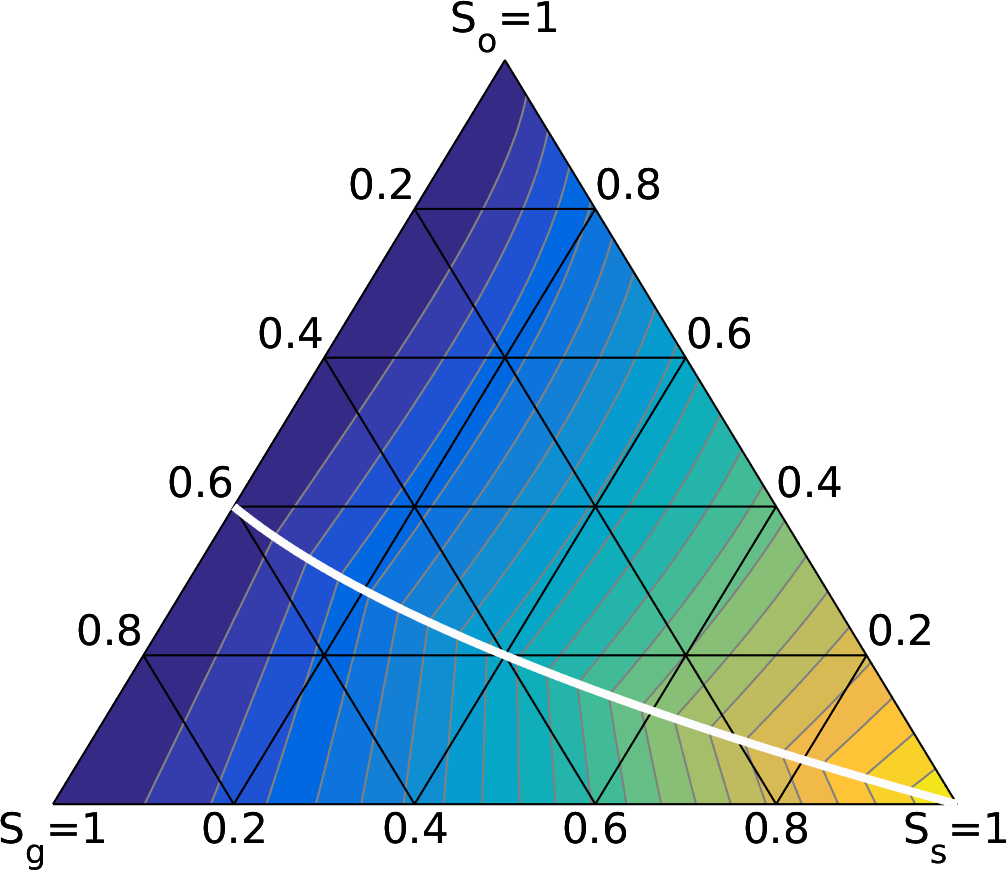
\includegraphics[width = 0.6\textwidth]{krS.png}};
  \node at (8.5,-5.5) {Solvent relperm};
  \node[anchor=south west,inner sep=0] (krG) at (0,0) {
    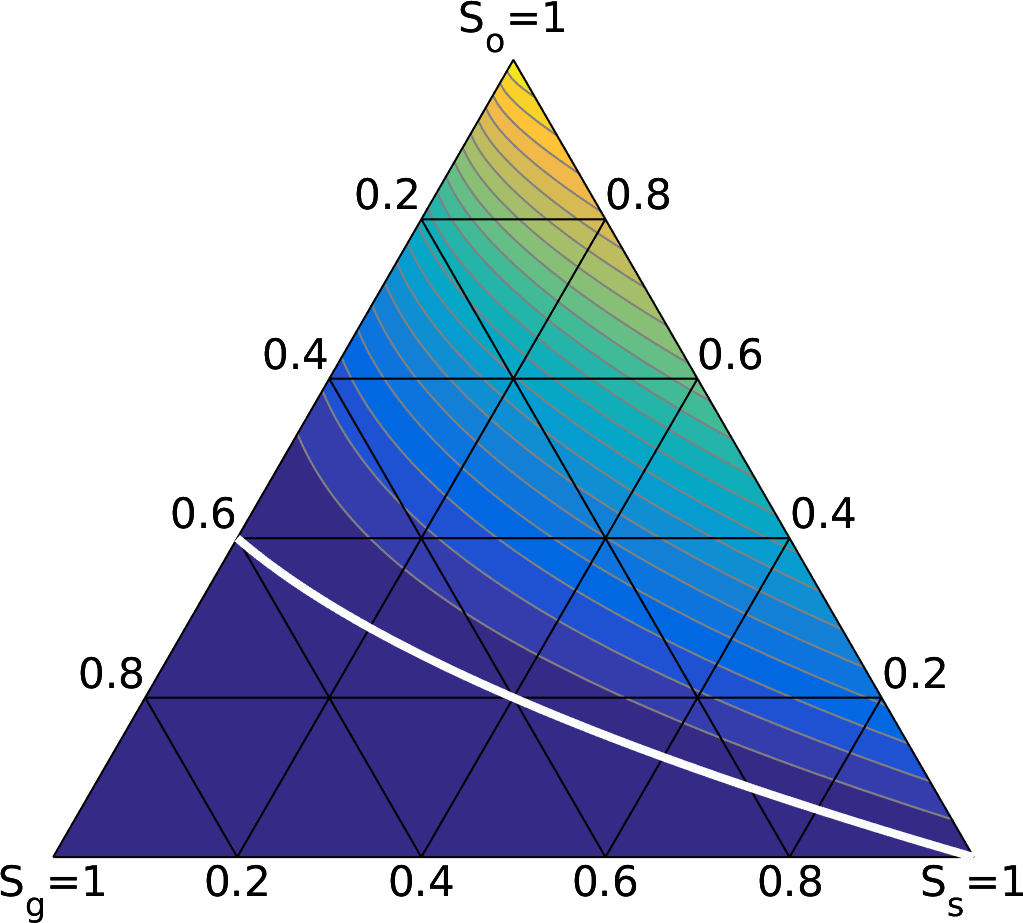
\includegraphics[width = 0.6\textwidth]{krO.png}};
    \node at (3.2,-0.5) {Oil relperm};
\end{tikzpicture}


\end{document}

%%% Local Variables:
%%% mode: latex
%%% TeX-master: t
%%% End:
